\documentclass[12pt,a4paper]{article}
\usepackage[utf8]{inputenc}
\usepackage[spanish]{babel}
\usepackage{amsmath}
\usepackage{amsfonts}
\usepackage{amssymb}
\usepackage{graphicx}
\usepackage[left=2cm,right=2cm,top=2cm,bottom=2cm]{geometry}

%--------------------------------------------------------%
%         Paquetes usados sólo para esta entrega         %
%--------------------------------------------------------%

\usepackage[hidelinks]{hyperref}
\usepackage{algorithm}
\usepackage{algorithmic}
\usepackage{float}




\author{Ignacio Aguilera Martos \\
	DNI: 77448262V       e-mail: nacheteam@correo.ugr.es}
\title{The Whale Optimization Algorithm \\ Metaheurísticas}
\date{Curso 2017-2018}

%Quita la sangría
\setlength{\parindent}{0cm}


\begin{document}
	\maketitle

	\tableofcontents

	\newpage

	%p 56

%	\framebox[16cm][c]{\LaTeX}

	\section{Introducción del problema}
	\label{sec:introProblema}
	
		Durante este trabajo he tenido como objetivo desarrollar un algoritmo mejorado a partir de un algoritmo bioinspirado de partida. Este algoritmo ha sido 'The Whale Optimization Algorithm' desarrollado y estudiado por los investigadores Seyedali Mirjalili y Andrew Lewis ambos de la universidad de Griffith.
		
		Para la comparativa y estudio de los resultados hemos puesto nuestro algoritmo a calcular los mínimos de 20 funciones. Estas funciones son las mismas que se utilizaron en la competición CEC2014, competición que pasaré a comentar brevemente en la siguente sección.
	
	\subsection{Competición CEC2014}
	
		Esta competición es un referente a nivel mundial en cuanto a competiciones de algoritmos se refiere. La intención de la competición es poner todos los algoritmos a ejecutar con diferentes dimensiones: 10,30,100,... de forma que se puedan comparar a posteriori los resultados obtenidos por los mismos.
		
		El problema consiste en minimizar 30 funciones que a priori no tienen un mínimo fácilmente localizable, como única garantía se tiene que el mínimo está localizado en el compacto $[-100,100]^n$ donde n es la dimensión considerada.
		
		En esta competición del año 2014 se evaluaron las funciones en dimensión 10,30,50 y 100 pero en este trabajo sólo hemos abarcado el problema de dimensión 10 y 30. Además cabe destacar que el algoritmo ganador en la competición fue L-SHADE.
	
	\subsection{Módulo de funciones CEC2014}
	
		Para poder ejecutar el algoritmo diseñado sobre las funciones de la competición CEC2014 primero tenemos que tener una implementación de las mismas. Mi decisión fue utilizar Python para el desarrollo del algoritmo, por la rapidez y facilidad en la escritura y sintaxis y por disponer de bibliotecas muy potentes en las que poder apoyar mi código.
	
		La implementación de las funciones nos fue dada en C++, por lo que tuve que hacer un módulo en Python primero que importase las funciones de C++ para poder utilizarlas en Python. Este trabajo lo hice de forma conjunta con mi compañero Pablo Baeyens utilizando la biblioteca Cython. Tras esto implementamos dos interfaces muy sencillas que permiten ejecutar las primeras 20 funciones de la competición a través de una clase Benchmark.
		
		Cabe destacar que esta idea se me ocurrió tras ver que el profesor de la Universidad de Granada en Ceuta Daniel Molina había desarrollado un módulo parecido para la competición de 2013 \cite{danielMolinaCEC2013}. Tras contactar con el y apoyarnos en su código terminamos de desarrollar el módulo de las funciones y lo subimos a GitHub dejándolo a disposición del resto de alumnos junto con el código de otro compañero que realizó el mismo trabajo para el lenguaje Julia \cite{cec2014github}.

	\newpage

	\section{Descripción del algoritmo inicial}
	\label{sec:descripcionAlgoritmoInicial}
	
		En esta sección vamos a pasar a describir con detalle el algoritmo inicial propuesto por Mirjalili y Lewis en su artículo \cite{paperWOA} desgranando cada elemento que pueda resultar interesante para el desarrollo de la explicación de las siguientes versiones.
	
	\subsection{Inspiración en la ballena jorobada}
	
		Este algoritmo basa su comportamiento en la naturaleza, por lo que es uno de los llamados algoritmos bioinspirados. En concreto en este caso el algoritmo toma como idea la forma en que las ballenas jorobadas se aproximan a su comida.
		
		Estas ballenas tienen dos formas comunes de alimentarse: aletear sobre sus presas y después comérselas o realizar un camino ascendente hacia ellas en forma de espiral para así concentrar los peces en la parte superior de la misma mientras que expulsan burbujas para aturdir a sus presas.
		
		Mediante estas dos formas de caza se están describiendo dos formas de aproximarse hacia las presas que en nuestro caso serán dos soluciones, por lo que con esto tendremos una aproximación lineal hacia la solución lo que nos va a dar en teoría una buena convergencia y tendremos una aproximación en espiral que intentará que no nos quedemos encerrados en mínimos locales ya que estaremos explorando un entorno de la solución cada vez más pequeño.
	
	\subsection{Modelo matemático}
	
		Para la descripción del modelo vamos a definir $a\in \mathbb{R}$ como un número que se decrementa de forma lineal desde 2 hasta 0 y $r\in \mathbb{R}$ un vector aleatorio en el intervalo $[0,1]$.
		
		A partir de estos números reales podemos definir $C\in \mathbb{R}$ como $C=2\cdot r$ y $A \in \mathbb{R}$ como $A = 2\cdot a \cdot r - a$. Nótese que estas variables van dependiendo de los dos reales definidos previamente.
		
		Para el movimiento lineal vamos a definir $D\in \mathbb{R}$ como $D=|C\cdot X^*(t)-X(t)|$ donde $X^*(t)$ es la posición de la mejor solución hallada hasta el momento y $X(t)$ es la posición actual de la ballena.
		
		Para el movimiento lineal con lo definido si estamos en la iteración t entonces obtenemos la posición de la siguiente iteración como:
		
		$$X(t+1) = X^*(t)-A\cdot D$$
		
		Donde el producto entre vectores se refiere al producto elemento por elemento y el producto de escalar por vector es el definido en un espacio vectorial cualquiera.
		
		Esta aproximación hecha hasta el momento es la lineal, la cual es la más sencilla de las dos y nos da el comportamiento más simple. Ahora vamos a desarrollar el movimiento espiral.
		
		Si nos fijamos en la variable A podemos ver que en realidad es un valor aleatorio en el intervalo $[-a,a]$ lo que nos permite que en cada iteración podamos tomas como siguiente punto cualquiera de los que se encuentran en el segmento que une $X(t)$ con $X^*(t)$.
		
		Para la aproximación en espiral definimos la constante real $b\in \mathbb{R}$ que que nos da la forma concreta de la espiral, en el caso del algoritmo implementado para el paper $b=1$. También definimos la variable $l\in \mathbb{R}$ que es un valor aleatorio en el intervalo $[-1,1]$.
		
		En este caso definimos también una variable dependiente de la posición actual y la mejor hasta el momento $D'\in \mathbb{R}$ como $D' = |X^*(t)-X(t)|$.
		
		Con todo lo definido la expresión del movimiento en espiral para la siguiente iteración t+1 viene dada por:
		
		$$X(t+1) = D'\cdot e^{bl}\cdot \cos(2\pi l) + X^*(t)$$
		
		Tras esto ya tenemos definidos los dos tipos de movimientos con las ecuaciones que los modelan. El comportamiento real del algoritmo va a depender de un valor aleatorio $p\in [0,1]$ de forma que:
		
		$$X(t+1) = 
		\begin{cases}
			X^*(t)-A\cdot D & si \ p<0.5\\
			D'\cdot e^{bl}\cdot \cos(2\pi l)+X^*(t) & si \ p\geq0.5
		\end{cases}$$
		
		A esto le sumamos el hecho de que en un estado inicial del algoritmo, o lo que es lo mismo si $|A|>1$, tenemos que en vez de dirigirnos hacia la mejor ballena hasta el momento nos vamos a dirigir a una posición aleatoria, de forma que vamos a ensalzar la exploración sobre la convergencia. Todas las fórmulas permanecen igual salvo que $X^*$ en este caso es un $X_{rand}$ aleatorio.
		
		\begin{figure}[!h]
			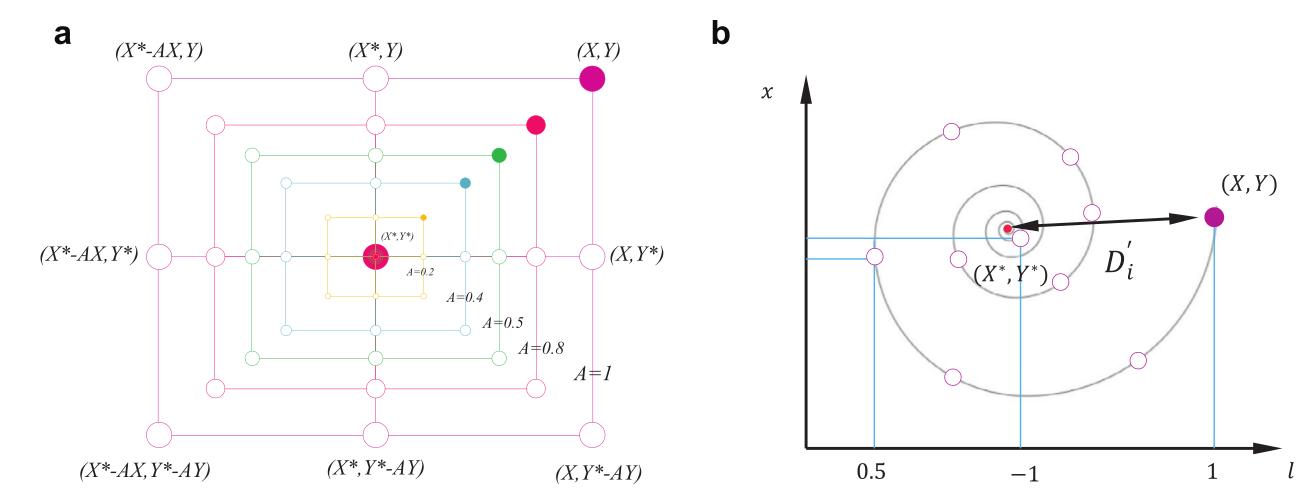
\includegraphics[scale=0.35]{./Imagenes/lineal_espiral.png}
			\caption{a) Aproximación lineal. b) Aproximación en espiral.}
		\end{figure}
		
	\subsection{Pseudocódigo del algoritmo}
	
		\begin{algorithm}[!h]
			\begin{algorithmic}[!h]
				\STATE Inicialización de la población de ballenas $X_i$ : $i=1,2,...,n$
				\STATE Se calcula el fitness de cada ballena.
				\STATE $X^*=$ la mejor de las ballenas.
				\STATE t=0
				\WHILE{t<máximo de iteraciones}
					\FOR{$X_i$ con i=1,2,...,n}
						\STATE Actualiza a,A,C,l y p (b=1).
						\IF{$p<0.5$}
							\IF{$|A|<1$}
								\STATE Actualiza la posición de la ballena $X_i$ utilizando la aproximación lineal con $X^*$
							\ELSE
								\STATE Escogemos una ballena aleatoria $X_{rand}$
								\STATE Actualiza la posición de la ballena $X_i$ utilizando la aproximación lineal con $X_{rand}$
							\ENDIF
						\ELSE
							\STATE Actualiza la posición de la ballena de forma espiral con $X^*$
						\ENDIF
					\ENDFOR
					\STATE Comprobar si alguna ballena se ha salido del espacio de búsqueda.
					\STATE Calcular el fitness de las ballenas de nuevo.
					\STATE Actualizar $X^*$
					\STATE t=t+1
				\ENDWHILE
				\RETURN $X^*$
			\end{algorithmic}
		\end{algorithm}
	
	\newpage
	
	\section{Desarrollo de mejoras}
	\label{sec:desarrolloMejoras}
	
	\subsection{Versión original}
	
	La primera aproximación al algoritmo implementado vino dada por la propia de los autores, realizada en el lenguaje Matlab y que yo tuve que adaptar a Python. Esta adaptación fue instrucción a instrucción para que el algoritmo se viera reflejado fielmente.
	
	La primera versión contiene el mismo esquema que el pseudocódigo mencionado con anterioridad pero si lo analizamos un poco mejor podemos ver que la población inicial no se genera de forma aleatoria como cabría esperar, si no que se inicializa con el vector $(0,...,0)$. Este hecho me resultó curioso cuando me di cuenta de que las funciones que se analizaban para el algoritmo tenían casi todas su mínimo en el 0. Por seguir unos propósitos más generales he decidido inicializar toda la población de forma aleatoria. En cuanto al resto del código no cambié nada puesto que quería mantener en un principio la esencia del algoritmo.
	
	\subsection{Aproximación espiral a una solución aleatoria}
	
	Para la segunda versión hice el primer cambio que comenté en la exposición de la metaheurística y que es evidente al mirar el algoritmo. Decidí meter también una búsqueda hacia una solución aleatoria si $|A|\geq 1$ en la espiral, de forma que en el primera fase del algoritmo se maximizara la búsqueda en el espacio de soluciones. Este cambio no resultó ser a mejor debido a que aunque en un principio pueda parecer lógico que el algoritmo así va a explorar más, con el tiempo y desarrollando versiones me dí cuenta de que lo que le faltaba al algoritmo no era más exploración o diversidad, si no convergencia como luego veremos.
	
	\subsection{Solis Wets}
	
	Para introducir la búsqueda local dentro del algoritmo y aportarle así un poco más de convergencia comencé implementado mi propia versión de la búsqueda local de forma parecida a cómo lo hemos hecho en las prácticas de la asignatura. Tomamos un vector de entrada y le realizamos una mutación en una de sus posiciones sumándole un valor generado por una distribución normal con $\mu = 0$ y $\sigma = 0.3$. Esto resultó ser una búsqueda local pésima que incluso era capaz de empeorar el algoritmo inicial por lo que la descarté.
	
	Tras esto acudí a los ficheros que se nos daban de ayuda, los cuales contenían una búsqueda local mucho mejor implementada en C++ pero de nuevo no me servían puesto que he realizado la implementación en Python. Acudí a la cuenta de GitHub de Daniel Molina y tras obtener su consentimiento he usado una implementación de la búsqueda local Solis Wets realizada en Python por él mismo \cite{solisWetsDanielMolina}.
	
	Esta búsqueda local se diferencia con respecto a la mía en tres aspectos. El primero de ellos es que añadido a sumar un incremento generado con una distribución normal tenemos el hecho de que se mantiene una inercia, es decir, si mejoramos el vector solución hacia una dirección concreta y nos estuvo dando éxito entonces continuaremos con una cierta inercia dirigiendo hacia allí la solución. El segundo aspecto es que si en una dirección de modificación del vector no estamos obteniendo mejoras entonces vamos a coger en la iteración siguiente justo la dirección opuesta. Por último el valor $\sigma$ de la distribución normal $\mathcal{N}(0,\sigma)$ se va incrementando o decrementando en función del número de éxitos al realizar la mejora, es decir, si superamos un umbral de éxitos incrementaremos el valor de $\sigma$ y si superamos un umbral de fallos entonces decrementaremos el valor de $\sigma$. 
	
	Con esta nueva búsqueda local realicé la tercera versión del algoritmo. La idea es que cada mil iteraciones introducimos una búsqueda local que nos va a favorecer la convergencia del algoritmo. Además para intentar mejorar lo máximo posible la solución reservo al final 1000 evaluaciones para que la búsqueda local pueda intentar mejorar el resultado del algoritmo. 
	
	Tras hacer esto de nuevo vi que la convergencia era demasiada, es decir, el algoritmo mejoraba muy rápido cuando se empleaba la búsqueda local pero en el resto del proceso no se mejoraba demasiado puesto que las ballenas acababan estando demasiado próximas entre sí. Por ello decidí meterle un esquema muy pequeño de mutación para que diversificara el proceso. En vez de realizar un movimiento en espiral decidí cambiarlo por una mutación del 20\% de la población volviendo a generarlos de forma aleatoria. Lo que conseguimos con esto es que la población vaya mejorando en términos generales, pero si entramos en la parte del algoritmo asociada a la espiral entonces mutamos para dar mas diversidad. Haciendo estos cambios como veremos posteriormente obtuve una mejora muy notoria en los resultados.
	
	\subsection{Differential Evolution}
	
    En la cuarta versión quise meter un esquema de diversidad un poco más elaborado que el de la tercera versión. Lo primero que hice fue cambiar el condicional sobre el valor aleatorio p. Ahora solo entraremos en la parte del condicional correspondiente a la espiral si $p\geq0.9$ lo cual reduce las posibilidades de entrar en la mutación.
    
    Para suplir este cambio le metí un esquema de differential evolution cada 10.000 iteraciones. Este esquema de differential evolution lo que hace es ejecutar un algoritmo de differential evolution durante un número de iteraciones concretas. La elección de este algoritmo fue los buenos resultados que obtenía en todos los rankings de competiciones de algoritmos, además disponía de él de forma fácil pues lo habíamos implementado en las prácticas y por tanto sólo tenía que adaptar mi código a es de este problema. Como esquema de mutación tomé el operador Rand1 que es el que mejores resultados me dió en la práctica comparado con Current to Best 1. Cabe recordar que el esquema de mutación toma para cada individuo a mutar tres individuos aleatorios de la población y mediante un factor F obtiene el vector mutado como:
    
    $$mutado = poblacion[rand_1] + F\cdot (poblacion[rand_2]-poblacion[rand_3])$$
    
    Donde la constante F es la recomendada en las diapositivas de teoría $F=0.5.$
    
    Tras esto me di cuenta de que los resultados del algoritmo no habían mejorado todo lo que esperaba. Esta mejora está claro que desarrolla más diversidad que convergencia con respecto al esquema de la búsqueda local, por lo que decidí que, además de cambiar el umbral de p a partir del cual entramos en la mutación del 20\% de la población, iba a realizar la mutación sobre el 20\% peor y no sobre un 20\% aleatorio. Tras este cambio mejoró un poco el algoritmo.
    
    \subsection{CMAES}
    
    Llegados a este punto el algoritmo mantenía un equilibrio entre convergencia y diversidad bastante ajustado, ya que añadiendo más evaluaciones a la búsqueda local o quitándole no conseguía una mejora sustancial. Por ello se me ocurrió que más que quitar o sumar evaluaciones a la búsqueda local lo que tenía que hacer era aprovechar mejor las evaluaciones que le estaba cediendo con respecto al resto del algoritmo.
    
    Por ello decidí utilizar un algoritmo más potente como CMAES. El problema que tuve con este algoritmo fue parecido al que he relatado previamente con la búsqueda local. En primer lugar intenté acudir de nuevo a Daniel Molina para ver si tenía una versión en Python de CMAES. Esta consulta resultó satisfactoria pues sí la tenía pero al comprobar con más detalle me dí cuenta de que estaba escrita en Python2 mientras que yo estaba empleando Python3 que no tiene retrocompatibilidad. Por ello volví a preguntarle y me sugirió que usase la implementación de los propios autores que tienen disponible en su GitHub \cite{PYCMA}.
    
    Esta implementación tiene su propia sintaxis para las funciones, por lo que tuve que modificar ligeramente los ficheros de CMAES hasta que pude hacer que funcionara con mi algoritmo. El cambio realizado por tanto fue reemplazar todas las búsquedas locales por llamadas a CMAES de forma que mejorase mucho más la solución en el mismo número de evaluaciones. Este cambio le dió una mejora sustancial a los resultados aunque ya estaba acercándome a los mínimos de las funciones.
    
    \subsection{Posición aleatoria}
    
    Por último, tras revisar el algoritmo en busca de posibles mejoras empecé a prestarle atención a la fase inicial del mismo. En la fase inicial el algoritmo en vez de aproximarse hacia la mejor ballena se aproxima a una de ellas escogida de forma aleatoria. Este comportamiento puede llevar a que las ballenas se acaben agrupando entorno a ellas mismas y por tanto arruinaría la exploración. Por ello el último cambio que he realizado al algoritmo ha consistido en hacer una aproximación a un vector aleatorio en vez de a una ballena aleatoria.
    
    Esta mejora que a priori pudiera parecer un tanto trivial mejoró la exploración del algoritmo tanto que en algunos casos mejoré 1000 unidades respecto a la versión anterior.
    
	
	\section{Versión final}
	\label{sec:versionFinal}
	
	\section{Resultados}
	\label{sec:resultados}
	
	%---------------------------------------------------------------------------------%
	
	%                               Bibliografía                                      %
	
	%---------------------------------------------------------------------------------%
	
	\newpage
	
	\bibliography{referencias} %archivo referencias.bib que contiene las entradas 
	\bibliographystyle{plain} % hay varias formas de citar

\end{document}
